% R1 in the Java engine: n-step targets with k branches per draw (examples.rl.CompareNStep).
% Figure from rl/experiments/plot_java_nstep.py; numbers from rl/experiments/results/java_nstep_compare.csv.

\subsection{R1 in the Java engine: n-step targets with $k$ branches (2026-10-14)}
\label{sec:java-nstep}

\note{\textbf{In short.} The same question, asked of the real engine rather than the Python prototype: does the
paratemporal engine help n-step Monte Carlo with $k$ branches per node? Yes. Merging makes a $k$-tree 5--10$\times$ more
efficient, and \textbf{budget reallocation with merging is the best sampled method in all 12 settings}, 1.2--2$\times$
more efficient than independent rollouts. Exhaustive expansion with merging gives the exact target at a cost close to a
single sampled estimate on the random walk, and 7$\times$ cheaper than unmerged exhaustive expansion on FrozenLake.}

\paragraph{Setup.} \code{examples.rl.MdpWalker} follows a fixed policy in a tabular MDP and draws its next state when it
\emph{leaves} a state, after the engine has merged the branches that reached it (``merge, then sample''). The n-step
expected target $E[\sum_{i\le n}\gamma^{i-1}R_i+\gamma^n V(S_n)\mid S_0=s]$ is computed with $V=V^\pi$, so every exact
target equals $V^\pi(s)$ and bias is measured against a known value. Problems: the 19-state random walk (5 start states)
and slippery FrozenLake $8\times8$ with the $\varepsilon$-soft optimal policy ($\varepsilon=0.2$, $\gamma=0.99$; 6 start
states); $n=2,4,6$; $k=2,3$; 200 replications per sampled method. Two new selection rules make this possible:
\code{SelectionRule.monteCarlo(k)} ($k$ samples per draw, weight $w/k$ each) and \code{SelectionRule.budget(B)}
($\max(1,\mathrm{round}(Bw))$ samples per draw for a branch of weight $w$). Work is the engine's departure count;
efficiency is variance $\times$ work (lower is better; for an unbiased estimator variance falls as $1/\text{work}$).

\begin{center}\small
\begin{tabular}{@{}lrrrr@{}}
\toprule
& \multicolumn{2}{c}{\textbf{Random walk}, $n=6$, $k=3$} & \multicolumn{2}{c}{\textbf{FrozenLake} $8\times8$, $n=6$, $k=3$}\\
\cmidrule(lr){2-3}\cmidrule(l){4-5}
\textbf{Method} & \textbf{Work} & \textbf{Var $\times$ work} & \textbf{Work} & \textbf{Var $\times$ work}\\
\midrule
$k$-tree, no merge & 2{,}132 & 10.9 & 1{,}812 & 0.616\\
$k$-tree + merge & 102 & 1.02 & 213 & 0.122\\
budget $B=9$ + merge & 82 & \textbf{0.546} & 85 & \textbf{0.042}\\
9 independent rollouts & 125 & 0.835 & 115 & 0.053\\
exhaustive, no merge & 249 & exact & 5{,}060 & exact\\
exhaustive + merge & 102 & exact & 730 & exact\\
\bottomrule
\end{tabular}
\end{center}

\begin{figure}[h]\centering
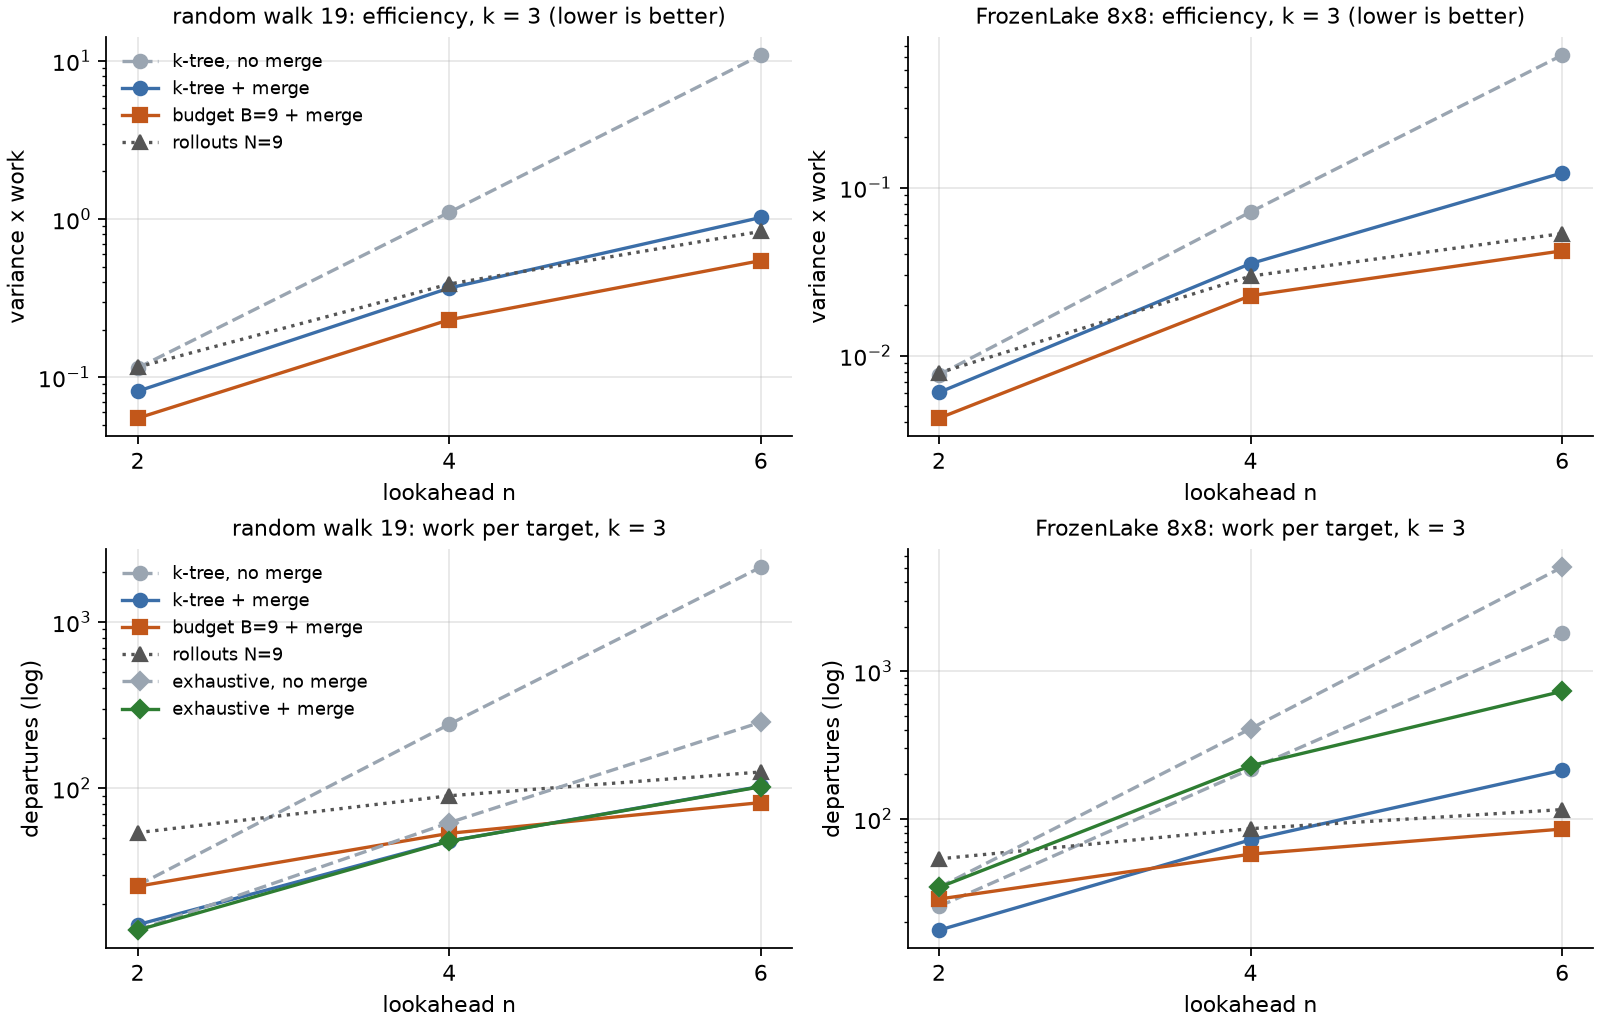
\includegraphics[width=\linewidth]{java_nstep_compare.png}
\caption[Java engine, k = 3: efficiency and work against lookahead]{Java engine, $k=3$: efficiency (top) and work
per target (bottom) against lookahead $n$. Full results for $k=2,3$ and $n=2,4,6$ are in
\protect\path{rl/experiments/results/java_nstep_compare.csv}.}
\end{figure}

\paragraph{What it shows.}
\begin{enumerate}
\item \textbf{All sampled estimators are unbiased}: every mean is within about 2 standard errors of the exact target.
\item \textbf{Merging a $k$-tree pays}: work falls 8--21$\times$ at $n=6$, $k=3$, variance rises only 1.5--2$\times$ (merged
  branches share one sampled future, as Section~\ref{sec:variance} predicts), so efficiency improves 5--10$\times$. The
  gain grows with $n$ and $k$; at $n=2$ there is little to merge.
\item \textbf{A merged $k$-tree with a fixed $k$ is still only level with independent rollouts}, and worse on FrozenLake
  at $n=6$. The fix is the one the variance analysis gives: \textbf{reallocate the budget by weight}. Budget + merge is
  the most efficient sampled method in every one of the 12 settings, 1.2--2$\times$ better than rollouts. Part of that
  edge is that the tree simulates the shared first steps once, where each rollout repeats them.
\item \textbf{Exact expansion is competitive.} On the random walk, exhaustive + merge costs about one sampled estimate
  and has no variance. On FrozenLake it costs 730 departures; at budget + merge's efficiency, any standard deviation
  below about $\sqrt{0.042/730}\approx0.008$ costs more than that by sampling, so exact wins whenever that precision
  is needed.
\end{enumerate}

\paragraph{Found and fixed along the way.}
\begin{itemize}
\item \textbf{Correlated seeds.} \code{java.util.Random} gives nearly equal first values for nearby seeds: across seeds
  $7,8,9,\dots$ the first draw from a 4-outcome law never produced one of the outcomes. Averages over replications
  seeded $1,2,3,\dots$ were therefore biased (all sampled estimators came out low, by up to 9 s.e.). The engine now
  passes the seed through a SplitMix64 scramble, so nearby seeds give independent streams.
\item \textbf{FrozenLake ground truth.} $V^*(\text{start})=0.414640361787$ at $\gamma=0.99$; the Java model and the
  Gymnasium-derived Python model agree to $10^{-11}$ (an earlier note of 0.542 was wrong).
\item \textbf{Results file.} Method names containing commas were written unquoted; the CSV writer now quotes text.
\end{itemize}

\paragraph{Checks.} \code{examples.rl.VerifyNStep} (22 checks, part of the build): exact targets equal $V^\pi(s)$ to
$10^{-12}$ with and without merging and with one or two draws per step, $V^*$ matches the Python value, merging reduces
work, and the four sampled estimators are unbiased within 4 s.e. \code{CompareNStep} runs its replications in parallel
(\code{-Dthreads}); results are identical for any thread count.

\paragraph{Caveats.} Both problems pay rewards only on arrival in end states, so safe merging fires; with a reward on
every step it needs the expectation-only merge (approved as an opt-in, in progress). These are prediction results for a
fixed policy; control is the next phase.
